%!TEX root = paper.tex
\begin{figure*}
	\begin{center}
		\subfloat[PC]
		{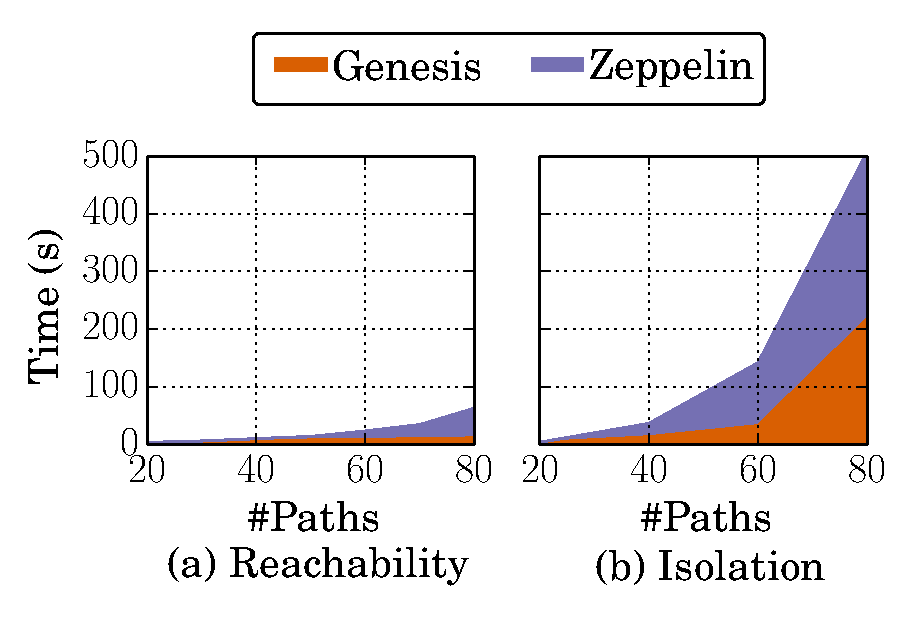
\includegraphics[width=0.33\columnwidth]{figures/ospfisolation.eps}}
		\subfloat[1-WC]
		{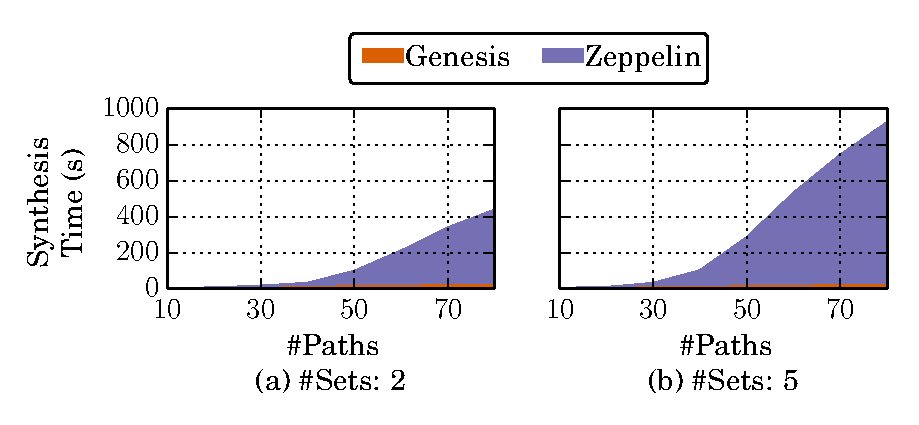
\includegraphics[width=0.325\columnwidth]{figures/ospfwaypoint.eps}}
		\subfloat[2-WC]
		{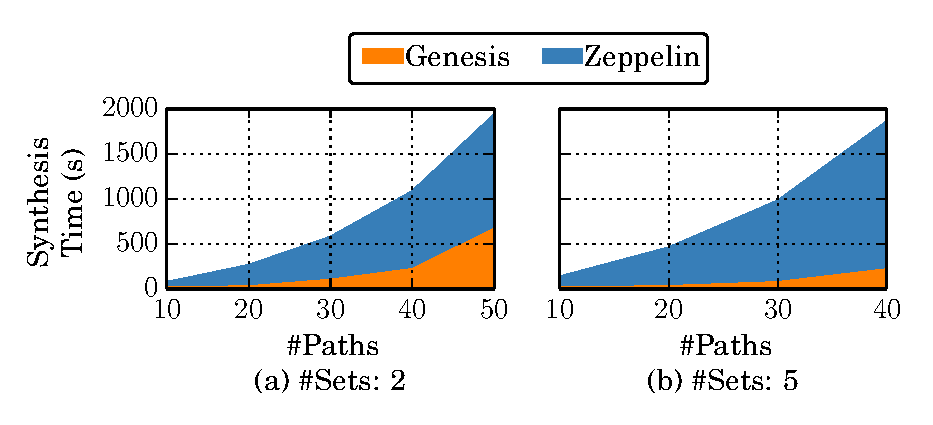
\includegraphics[width=0.33\columnwidth]{figures/ospfwaypoint2.eps}}
		\caption{\label{fig:ospfend2end}
			End-to-end synthesis time for waypoint policy workloads for varying 
			number of paths and different number of waypoint sets.}
	\end{center} 
\end{figure*}
\section{Evaluation}
 \label{sec:evaluation}
 We implemented a prototype of \name in Python. 
 For a given workload, \name outputs Quagga template
 configurations~\cite{quagga}. 
 We use the Gurobi solver~\cite{gurobi} 
 for linear constraints generated by \name.
  In this section, we evaluate \Name using
%\loris{really don't like the word realistic}
enterprise-scale data
center fat-tree topologies~\cite{fattree} of different 
sizes. Experiments were conducted on a
32-core Intel-Xeon 2.40GHz CPU machine and
128GB of RAM.
Specifically, we ask the following questions.

\vspace{2mm}
\noindent\textbf{Q1}: How does \name perform on different  workloads? (\secref{sec:ospfeval})\\
\noindent\textbf{Q2}: How resilient are \name's  configurations? (\secref{sec:reseval})\\
\noindent\textbf{Q3}: Can \name get higher resilience by trying different domain assignments? (\secref{sec:mcmceval})\\
\noindent\textbf{Q4}: How does \name compare with the state-of-the-art? (\secref{sec:synet})



\subsection{Single Domain End-to-end Performance}\label{sec:ospfeval}


We evaluate the end-to-end performance of our tool
on a  fat-tree 
topology with 45 routers
and a single OSPF domain. 
The size of the topology is consistent with operator preferences to restrict
the size of a domain to under 50 routers.
PC refers to the algorithm that handles complex policies and
synthesizes policy-compliant
configurations with few static routes (\secref{sec:config-synthesis})
and 
1-WC (resp. 2-WC) refers to the version of the algorithm that handles waypoint policies and
can synthesize policy-compliant
configurations with high policy-resilience from 1 path (resp. 2 paths) per waypoint policy (\secref{sec:waypointres}).

We consider two classes of policies. 
We evaluate algorithm PC to handle simple
reachability policies and complex isolation policies that 
existing tools cannot handle; 
Our second class consists of
 waypoint policies of the form described in ~\secref{sec:waypointres};
for this class we evaluate 1-WC and 2-WC.
For each algorithm we report the time for 
\genesis to generate policy-compliant forwarding paths
and time \name takes to generate configurations 
from these paths. We set a timeout of 2,000 seconds for each workload.

\minisection{Reachability Policies}
We generate reachability policies (each of which 
corresponds to a path) with randomly generated endpoints.
\Cref{fig:ospfend2end}(a)(a) shows the synthesis time for
PC for varying number of paths. 
For these workloads, \name can
synthesize configurations for 80 policies in 62 
seconds, out of which configuration synthesis from paths 
takes 52 seconds on average.

\minisection{Isolation Policies}
We generate policies to ensure tenant-isolation
in a multi-tenant topology, i.e., each
tenant's traffic will be isolated from traffic from
other tenants, and a tenant cannot interfere with any 
other tenant. This is achieved by adding isolation policies
amongst different tenant's traffic. 
We have $n$ tenant groups (between 1 to 4), 
each group comprised of $g$ destinations (20). 
\Cref{fig:ospfend2end}(a)(b)
shows the synthesis time 
for PC.
The x-axis shows the paths $n * g$. 
 
 % \begin{figure}
 %  	\vspace{-4mm}
 % 	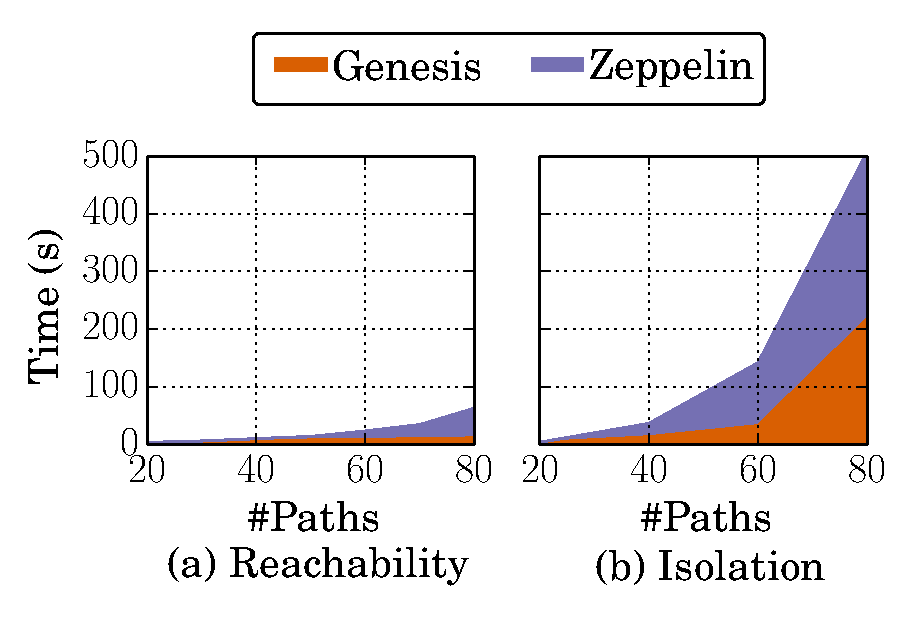
\includegraphics[width=\columnwidth]{figures/ospfisolation.eps}
 % 	\vspace{-8pt}
 % 	\caption{\label{fig:ospfisolation}
 % 	 Synthesis time for reachability and isolation workloads.}
 % \end{figure}
 

As the number of tenants increase, time to 
synthesize the data plane increases exponentially 
because finding isolated paths is NP-complete. Also, these
paths are longer than if we only had reachability policies. 
Similarily, time taken to synthesize 
OSPF configurations increases exponentially with the 
number of tenants as PC needs to add more static routes 
and requires more iterations of the unsat-core learning
procedure. 
For this workload, \name can
synthesize configurations for 4 tenants, each with
20 destinations in 507 seconds, where \genesis takes 217 seconds
for synthesizing paths. Note that synthesizing 
configurations is harder for isolation than reachability 
because of longer paths provided by Genesis.

\minisection{Waypoint Policies}
We generate waypoint policy 
workloads with varying number of destination subnets and 
waypoint sets as follows. 
We consider workloads with 2 and 5 unique waypoint 
sets where each set contains 3 randomly picked routers.  
Each waypoint set can be 
viewed as a class of replicated middleboxes.
We randomly generate policies 
that map each subnet to one of the waypoint sets. 

%Genesis generates a single path for each 
%destination, and \name synthesizes waypoint-compliant OSPF 
%configurations ((referred to as 1-WC) ) 
%using the waypoint policies and paths generated by Genesis.  
\begin{figure*}
	\centering
	\subfloat[2-WC vs. PC]
	{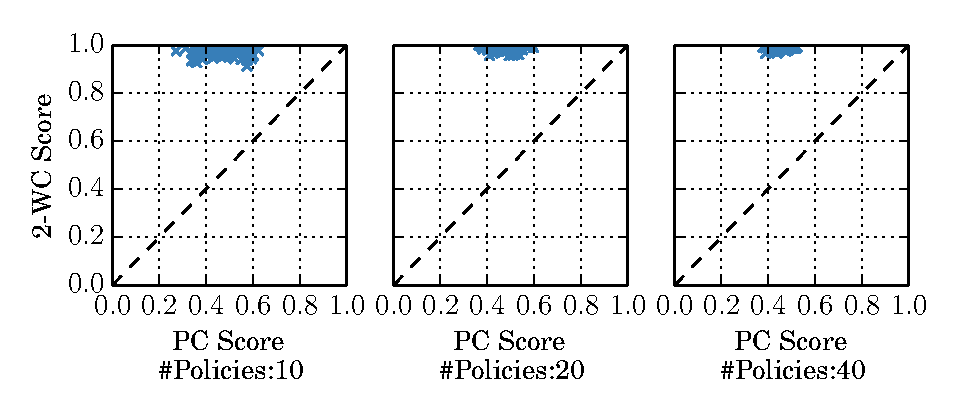
\includegraphics[width=0.49\columnwidth]{figures/ospfresilience2.eps}}
	\subfloat[2-WC vs. 1-WC]
	{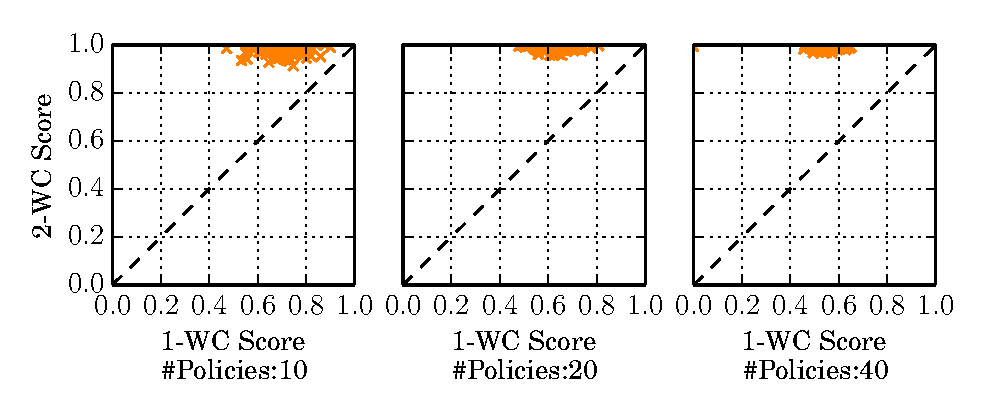
\includegraphics[width=0.5\columnwidth]{figures/ospfresilience.eps}}
	%	\subfloat[Number of Route Filters]
	%	{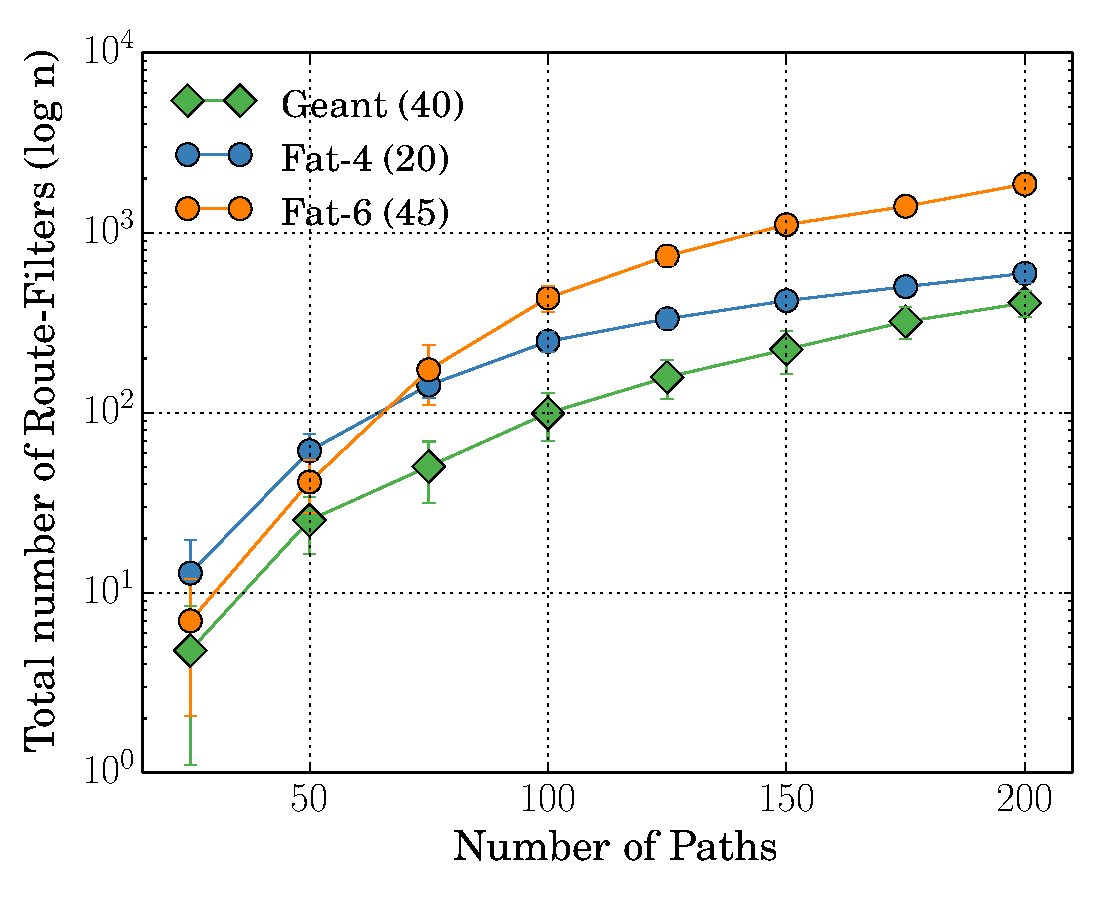
\includegraphics[width=0.33\columnwidth]{figures/ospfRF.eps}}
	%	\subfloat[Endpoint Resilience]
	%	{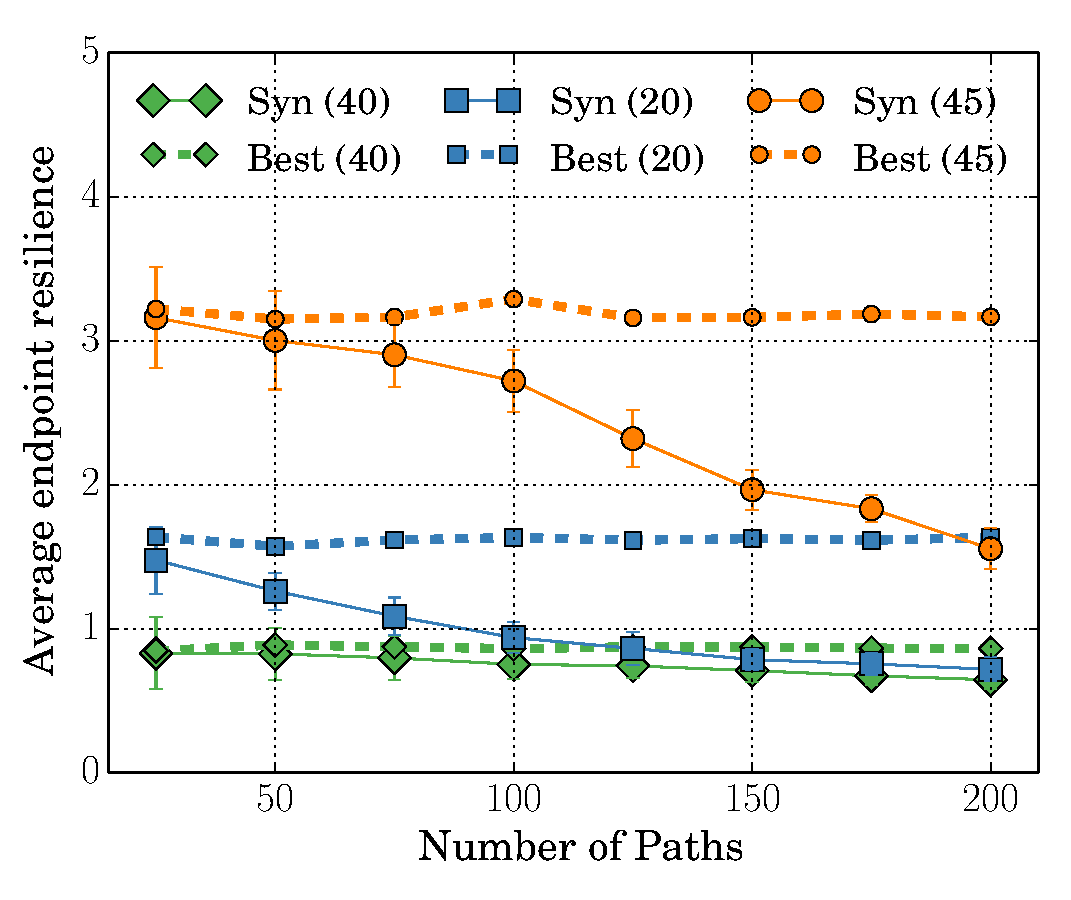
\includegraphics[width=0.32\columnwidth]{figures/ospfAvgRes.eps}}
	\caption{\label{fig:ospfres}
		Policy-resilience scores of 2-WC, 1-WC, and PC synthesis 
		for varying waypoint workloads.}
\end{figure*}

\Cref{fig:ospfend2end}(b) and (c) show the end-to-end synthesis
 time for varying number of destination paths and the 
 number of unique waypoint sets (2 and 5). 
 Since synthesizing paths
 for waypoint policies can be done independently,
Genesis synthesis time is small compared to OSPF synthesis. 
The synthesis times of 1-WC and 2-WC 
increase with the number of waypoint sets because
the algorithms 
need to add constraints corresponding to $D(s,t,\waypt)$ 
for each set. Hence, computing the unsat-core in each
iteration to find static routes is more expensive. 
For 5 waypoint sets and 40 destinations, \name takes 120 
seconds on average to synthesize waypoint-compliant configurations
and 1800 seconds to synthesize policy-resilient configurations.

\textbf{Q1:} \textbf{\name can synthesize policy-compliant configurations for medium size topologies} in less than 10 minutes and policy-resilient 
configurations in  less than an hour.

%\begin{table}{l}{8em}
%	\begin{footnotesize}
%		\begin{center}
%			\begin{tabular}{P{10em}| P{4em} | P{4em} | P{4em} | P{4em}}
%				Synthesis Type & Number of Packet Classes & Avg. Synthesis time (s) & Avg. Number of Resilient Classes & Ratio of Static Routes \\
%				\hline
%				1-Resilient Waypoint & 10 & 122.16 & 7.13 & 7/100\\
%				Waypoint & 10 & 7.85 & 0.3 & 7/100\\
%				1-Resilient Waypoint & 20 & 122.16 & 7.1 & 7/100\\
%				Waypoint & 20 & 7.85 & 0.3 & 7/100\\
%				1-Resilient Waypoint & 40 & 122.16 & 7.1 & 7/100\\
%				Waypoint & 40 & 7.85 & 0.3 & 7/100\\
%			\end{tabular}
%		\end{center}
%		\caption{Average synthesis time per class for waypoint policies with increasing number of waypoints. } \label{tab:waypointeval} 
%	\end{footnotesize}
%\end{table} 


\subsection{Resilience of Intra-domain Configurations} \label{sec:reseval}



% \begin{wrapfigure}{r}{0.42\columnwidth}
% 	% \vspace{-6mm}
% 		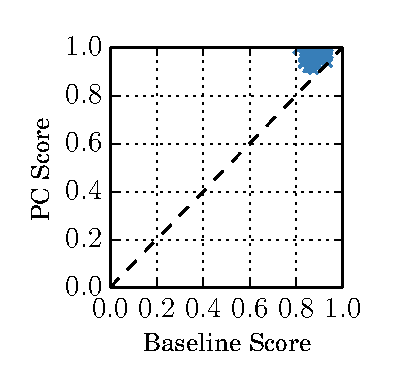
\includegraphics[width=0.4\columnwidth]{figures/ospfbaselineresilience.eps}
% 		\caption{
% 		Connectivity-resilience: PC vs baseline.}				
% \end{wrapfigure}

\minisection{Connectivity-resilience}
We measure the connectivity-resilience of the configurations 
generated using the algorithm PC on the reachability 
workload described in
Section~\ref{sec:ospfeval}. 
\begin{wrapfigure}{r}{0.33\columnwidth}
	\resizebox {0.33\columnwidth} {!} {
		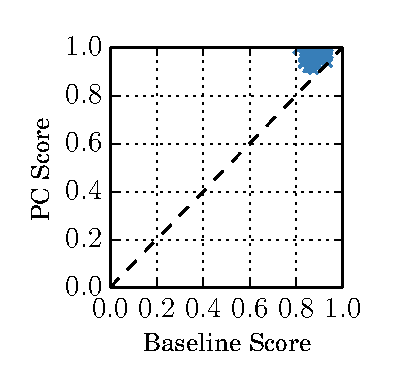
\includegraphics[width=0.44\columnwidth]{figures/ospfbaselineresilience.eps}
	}
	\caption{Connectivity-resilience: PC vs baseline.}
	\label{fig:ospfresbaseline}
\end{wrapfigure}
For our baseline, we use configurations 
where paths 
are enforced using only static routes and
OSPF weights are assigned randomly.
\Cref{fig:ospfresbaseline}
shows the results. 
A point above the diagonal 
denotes a benchmark in which \name
generated a configuration with higher connectivity resilience than
the baseline algorithm.
PC provides an average connectivity-resilience score 
of 0.97 over the baseline score 
of 0.88.
Moreover, PC places on average 
$9.3$\% of the static routes 
than required by the baseline. 

\minisection{Policy-resilience}
We measure the policy-resilience of the configurations 
generated using algorithms  1-WC and 2-WC on the waypoint workload described in
\secref{sec:ospfeval} with 5 waypoint sets. 
For each workload, we run each algorithm 
3 times with a different random seed, and report the most-resilient configuration it obtains.
For our baseline, we use the configurations generated by the algorithm PC, which
only tries to reduce the number of static routes.

\Cref{fig:ospfres}
shows the results
for varying number of policies (10, 20 and 40), each policy mapped 
to a particular destination IP address. 
For the plot on the left (resp. right)
a point above the diagonal 
denotes a benchmark in which 2-WC
generated a configuration with higher policy-resilience than
PC (resp. 1-WC).
For 40 policies, 
2-WC can synthesize 
configurations with high policy-resilience
(average 0.98) over PC (average 0.41) and 1-WC (average 0.51). 
Although not as good as 2-WC, 1-WC is able to provide 
higher policy-resilience than
PC thanks to the relaxed constraints that do not require
the path given by \genesis to be the shortest one.

\textbf{Q2:} 
\textbf{\name can synthesize highly resilient configurations}.

% \begin{figure}
% \centering
% \begin{minipage}{.5\textwidth}
%   \centering
%   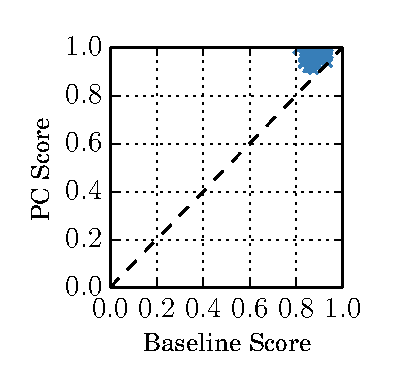
\includegraphics[width=.6\linewidth]{figures/ospfbaselineresilience.eps}
%   \captionof{figure}{Connectivity-resilience: PC vs baseline.}
%   \label{fig:ospfresbaseline}
% \end{minipage}%
% \begin{minipage}{.5\textwidth}
%   \centering
%   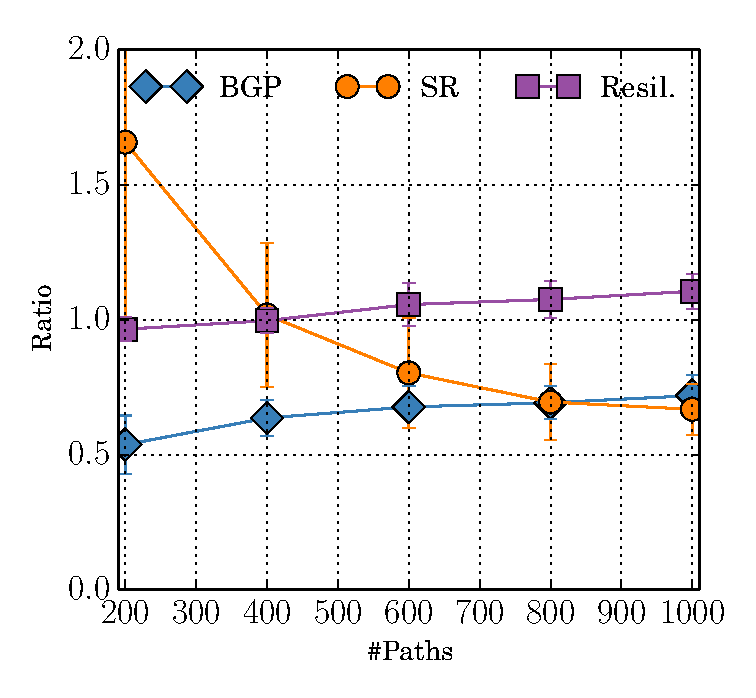
\includegraphics[width=.6\linewidth]{figures/ratioMCMC.eps}
%   \captionof{figure}{MCMC Evaluation for varying number of paths.}
%   \label{fig:mcmceval}
% \end{minipage}
% \end{figure}

\subsection{Dynamic Domain Assignment Performance} \label{sec:mcmceval}

In this section, we measure whether
when \name  is allowed to explore different domain assignments,
the MCMC algorithm presented in \secref{sec:synth-dom-ass}
can 
generate configurations
with higher resilience.
\begin{wrapfigure}{r}{0.45\columnwidth}
	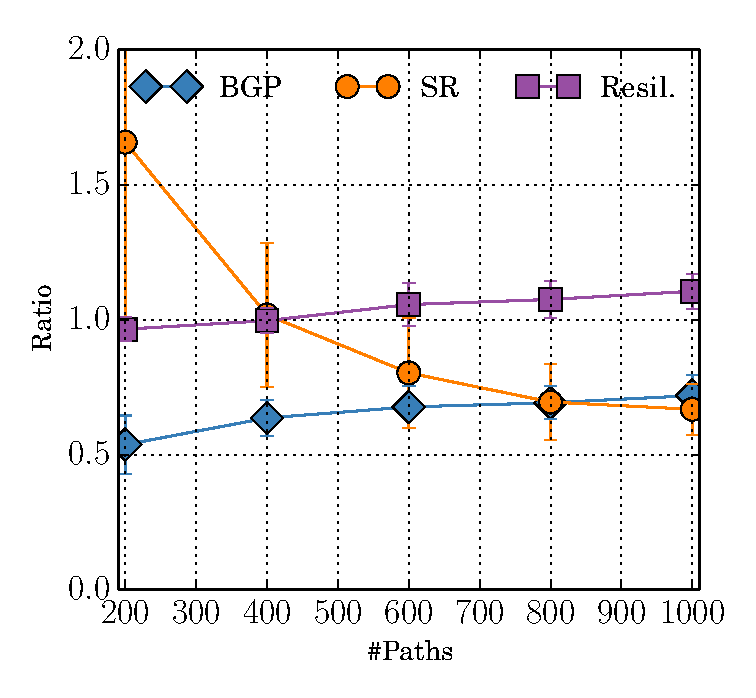
\includegraphics[width=0.45\columnwidth]{figures/ratioMCMC.eps}
	\vspace{-3mm}
	\caption{\label{fig:mcmceval}
		MCMC Evaluation for varying number of paths.}
\end{wrapfigure} 
We consider an 80 router fat-tree topology and run the MCMC sampling
for 600s---i.e., more than 100,000 iterations---to minimize the
 cost function $max(sc, bc)$. Using this cost function, \name
 tries to jointly decrease number of 
 BGP local preferences and static routes. 
 For the input, we generate $n$ (between
200 and 1,000) random paths for $n/4$ destination IPs, with random
path length between 3 and 10.  We require \name to split the network
into 5 OSPF domains each with size in range between 4 and 10.
We conduct each experiment 20 times and report averages and standard
deviations.  For each MCMC run, we collect the domain assignments with
worst and best scores.  For these assignments, we use the algorithm PC
to compute path-compliant configurations.
%We also store the worst configuration in terms of either
%configuration overhead $bc$ and the static route cost 
%$sc$. 
\Cref{fig:mcmceval} shows, for varying number of paths, the average ratios
between the best- and worst-score configurations
in terms of
BGP configuration overhead, 
number of static routes, and 
connectivity-resilience.
For smaller workloads, 
the algorithm reduces the BGP configuration overhead, but increases 
static routes, leading to worse connectivity-resilience. For 
larger workloads, the algorithm can
reduce both static routes 
and BGP local preference entries by $0.3\times$
and improve the connectivity-resilience 
by $0.1\times$.

\textbf{Q3:}
When allowed to try different domain assignments,
\textbf{\name synthesizes configurations with higher connectivity-resilience mainly for workloads with large number of paths}.

\subsection{Comparison to SyNET}
\label{sec:synet}
SyNET~\cite{synet} is a network-wide configuration synthesis system 
which supports multiple routing protocols (OSPF and BGP) and static 
routes. In this section, we compare SyNET's performance with \name 
for OSPF + static route configuration synthesis workloads obtained from the 
authors of SyNET.

\begin{figure}
	\small
		\begin{minipage}{0.9\columnwidth}
			\centering
			\begin{tabular}{P{3.4em} P{3em} m{2.5em} m{3.5em} m{3.5em}} 
			{\bf Topology}& {\bf \#Classes} & {\bf SyNET} & {\bf Zeppelin} & {\bf Speedup} \\ 
				\hline
				\multirow{3}{*}{Internet2}& 1 & \hfill 9.0s & \hfill 0.02s &  \hfill \textbf{450$\times$} \\
				 & 5 & \hfill 21.3s &\hfill	0.03s &	\hfill\textbf{710$\times$} \\
				 & 10 & \hfill 49.3s & \hfill	0.03s &\hfill 	\textbf{1,643$\times$} \\ 
				\hline 
				\multirow{3}{*}{G3} &  1 & \hfill 9.4s & \hfill	0.03s &	\hfill \textbf{313$\times$}\\
				 & 5 & \hfill 19.8s &\hfill	0.03s &  \hfill \textbf{660$\times$}\\
				&  10 &  \hfill 39.9s	& \hfill 0.03s	& \hfill \textbf{1,330$\times$} \\ 
			\end{tabular}
		\end{minipage}
		\caption{
		Comparison of synthesis times of  
			\name and SyNET for OSPF + Static route workloads.  }
		\label{tab:synetcomparison}
\end{figure}


For these experiments, we use the two network topologies the SyNET's authors made 
available: (1) Internet2:
a US-based network with 9 routers, and (2) G3: A $3 \times 3$ grid
topology. The routing requirements define the forwarding behavior
for 1, 5, and 10 traffic classes as follows:
for each router and traffic class
the workload specifies the next-hop router and the protocol for 
forwarding: OSPF or static route. 
Thus, for a topology with $n$ routers and $m$ traffic classes, 
the workload contains $n \times m$ SyNET requirements. 
We 
combine these requirements to generate paths to provide as input 
for \name's OSPF synthesis. Since the workload specifies which
routers had static routes installed for the different classes, we 
add these static routes (and remove the corresponding constraints), 
and use the algorithm presented in 
Section~\ref{sec:ospf} to find the OSPF weights.

\Cref{tab:synetcomparison} shows \name outperforms SyNET 
for all the workloads and topologies, achieving a best case 1,643$\times$
speedup 
 for Internet2 topology with 10 traffic classes. 
 In each of these experiments, \name 
invokes the LP solver once and does not need to add more static routes
than specified in the input requirements, which matches with the SyNET 
output (if more static routes were required, SyNET would have returned 
no solution for these experiments). 

\textbf{Q4:} 
\textbf{\name is 
able to achieve 2-3 orders of magnitude speedup over state-of-the-art tools}.